\documentclass[12pt]{report}
\usepackage{flushend}
\usepackage{graphicx}
\usepackage[noadjust]{cite}
% \usepackage[toc,acronym,description,sort=def]{glossaries}
\usepackage[toc,acronym,sort=def]{glossaries}
\usepackage{sectsty}
\usepackage{setspace}
\usepackage{enumerate}
\usepackage{IEEEtrantools}
\usepackage{paralist}
\usepackage{chngcntr}
\usepackage{ftnxtra}
\usepackage{amsmath}
\usepackage{algorithm}
\usepackage[noend]{algpseudocode}
\counterwithout{footnote}{chapter}
%\usepackage[top=1.4 in]{geometry}
\algnewcommand{\LeftComment}[1]{\Statex \(\triangleright\) #1}
\renewcommand{\bibname}{References}
\renewcommand{\algorithmicrequire}{\textbf{Input:}}
\renewcommand{\algorithmicensure}{\textbf{Output:}}
\chapterfont{\centering}
\pagestyle{headings}
\onehalfspacing

%************Glossary*************%

\makeglossaries

\newglossaryentry{dna}
{
    name=DNA,
    description={Deoxyribo Nucleic Acid, a molecule that codes genetic instructions in living organisms. It is a \emph{string} of 4 `nucleotides' - Nitrogen containing bases: Cytosine (C), Guanine (G), Adenine (A), and Thymine (T)}
}

 
%********End of Glossary**********%

\begin{document}

\begin{titlepage}
\begin{center}
\vspace{1cm}
\huge
\textbf{DNN Compiler for Custom AI Chip ISA}\\

\normalsize
\textbf{CS4099 Project Final Report}\\
\vspace{1cm}
\emph{Submitted by}\\        
\vspace{0.5cm}
\begin{tabular}{ccc}
\textbf{Mohammed Ameen }&& \textbf{B210515CS}\\
\textbf{Vivek K P}&& \textbf{B210473CS}\\
\textbf{Adil Abdul Jabbar}&&\textbf{B210461CS} \\
%\textbf{Name4}&&\textbf{Reg No: 4} \\
\end{tabular}\\
\vspace{0.8cm}
\textbf{Under the Guidance of\\Dr. Nirmal Kumar Boran}\\
\vspace{0.8cm}
\begin{center}
 
\includegraphics[width=0.2\textwidth]{nitc-logo.png}
\end{center}
\vspace{0.8cm}
\textbf{Department of Computer Science and Engineering}\\
\textbf{National Institute of Technology Calicut}\\
\textbf{Calicut, Kerala, India - 673 601}\\
\vspace{0.8cm}
\textbf{April 15, 2025}
\end{center}
\end{titlepage}
\pagenumbering{roman}
\begin{spacing}{1.01}
{
\thispagestyle{empty}

\fontsize{14}{14}\selectfont
\centering{\MakeUppercase{\textbf{National Institute of Technology Calicut, Kerala, India - 673 601}}} \\
\vspace*{0.5cm}
\fontsize{12}{12}\selectfont
\centering{\MakeUppercase{\textbf{DEPARTMENT OF COMPUTER SCIENCE AND ENGINEERING}}} \\
\begin{figure}[ht]
{\centering {
\includegraphics[width=0.2\textwidth]{nitc-logo.png}}\par}
\end{figure}
2025\\
\vspace{0.5cm}
\fontsize{14}{14}\selectfont
\textbf{\centering{CERTIFICATE}}\\
\vspace{0.25cm}
\fontsize{12}{12}\selectfont
\onehalfspacing{\textit{Certified that this is a bonafide record of the project work titled}}\\
\vspace*{0.25cm}
\textbf{\MakeUppercase{DNN Compiler for Custom AI Chip ISA}}\\
\vspace*{0.25cm}
\onehalfspacing{\centering{\textit{done by}}}\\
\vspace*{0.25cm}
\begin{tabular}{ccc}
\textbf{Mohammed Ameen }\\
\textbf{Vivek K P}\\
\textbf{Adil Abdul Jabbar}\\
%\textbf{Name4} \\
\end{tabular}\\
\vspace*{0.25cm}
\onehalfspacing{ \textit{\centering{of eighth semester B. Tech in partial fulfillment of the requirements for the award of the degree of Bachelor of Technology in Computer Science and Engineering of the National Institute of Technology Calicut}}}\\
\vspace*{0.5cm}
\noindent{
\begin{tabular}{p{4.8cm}cp{4.5cm}}
\textbf{Project Guide}  & \hfill \textbf{Head of Department} \\
Dr. Nirmal Kumar Boran & \hfill Dr. Subashini R\\
Assistant Professor & \hspace{5cm} Associate Professor\\
 & & \\
 & & \\
  & & \\

\end{tabular}
}
}
\chapter*{DECLARATION}
We hereby declare that the project titled, \textbf{DNN Compiler for Custom AI Chip ISA}, is our own work and that, to the best of our knowledge and belief, it contains no material previously published or written by another person nor material which has been accepted for the award of any other degree or diploma of the university or any other institute of higher learning, except where due acknowledgement and reference has been made in the text.\\

\vspace{2cm}
\noindent{
\begin{tabular}{p{8cm}p{6cm}}
Place :  & Signature : \\
Date : & Name : \\
 & Reg. No. : 
\end{tabular}
}
\newpage 

\begin{abstract}
Our project focuses on developing a DNN compiler that translates deep neural network models from Python-based AI frameworks to a custom AI chip’s Instruction Set Architecture (ISA), designed by the \textbf{Indian Space Research Organization (ISRO)}. The compiler converts models, built and trained using libraries like TensorFlow and PyTorch, into optimized machine instructions executed by the custom ASIC

The ASIC features a CISC-style ISA, capable of performing neural network operations like convolution and pooling with just a few instructions. The compiler is responsible for extracting layer-wise information, generating instructions for each layer, managing data dependencies, and optimizing memory usage. It also handles weight extraction, preprocessing, and memory arrangement to match the chip’s expectations.

This project contributes to ISRO’s larger vision of deploying custom ASICs in future space missions for tasks like real-time image processing and AI inference, where such chips outperform conventional GPUs under strict constraints like power limitations and harsh environments.

\end{abstract}
\chapter*{\rm \large \bf ACKNOWLEDGEMENT}
It is with immense gratitude that we acknowledge the support and guidance received from several individuals, without whom the successful completion of this project would not have been possible.

First and foremost, we would like to express our sincere thanks to \textbf{Dr. Nirmal Kumar Boran}, our project guide, for his invaluable encouragement, continuous support, and insightful guidance throughout the course of this work. His expertise and mentorship played a pivotal role in shaping the direction and outcome of our project.

We are also deeply grateful to \textbf{Dr. Chandramani Chaudhary} Assistant Professor, whose active involvement, thoughtful suggestions, and participation in our discussions greatly enriched this project. Her consistent support and encouragement have been of immense value.

We extend our heartfelt appreciation to \textbf{Piyush} and \textbf{Kaustab} from \textbf{URSC, ISRO}, key members of the ASIC chip development team, for their constant coordination, technical insights, and unwavering support in integrating our compiler with the hardware development process.

Finally, we thank all faculty members, peers, and family members who have directly or indirectly supported and encouraged us during this project.
\vspace{4.0mm}
\tableofcontents
\addtocontents{toc}{\vskip-30pt}
\end{spacing}
\listoffigures
\listoftables
\vspace{-2 em}
\printglossary[nonumberlist]


\pagenumbering{arabic}

\chapter{Introduction}

Artificial Intelligence (AI) has emerged as a transformative force in space exploration, enabling autonomous decision-making in critical applications such as satellite imaging, rover navigation, and real-time sensor data processing. Deep Neural Networks (DNNs), a subset of machine learning, have demonstrated exceptional performance in tasks like image classification, object detection, and signal processing. These networks mimic the human brain's structure, consisting of interconnected layers (e.g., convolutional, pooling, and fully connected layers) that extract hierarchical features from raw data through iterative training.

However, deploying AI models in space environments presents unique challenges. Space missions impose stringent constraints on \textbf{power consumption, size, weight, and radiation tolerance}, making conventional GPU-based inference systems impractical. General-purpose GPUs, while powerful, are energy-intensive and lack the ruggedization required for harsh space conditions. To address these limitations, specialized hardware solutions are essential.

The \textbf{Indian Space Research Organization (ISRO)} is pioneering the development of a \textbf{custom Application-Specific Integrated Circuit (ASIC)} tailored for AI inference in space. Unlike general-purpose processors, this ASIC is optimized to execute neural network operations\u2014such as convolutions, pooling, and dense layer computations\u2014with minimal power usage. Its \textbf{CISC-style Instruction Set Architecture (ISA)} is designed to perform these operations efficiently using a reduced instruction set, significantly lowering energy consumption compared to traditional GPUs.

A critical component of this system is the \textbf{memory hierarchy}, which includes:
\begin{itemize}
    \item \textbf{Frame Memory:} Stores intermediate feature maps generated during layer-wise processing.
    \item \textbf{Filter Memory:} Holds pre-loaded kernel weights for convolutional and dense layers, along with additional configuration parameters.
\end{itemize}

To further enhance efficiency, the ASIC makes use of \textbf{DSP parameters} (Digital Signal Processing parameters) during execution. These parameters enable the hardware to perform operations like \textit{bias addition and batch normalization} in a streamlined manner using a compact, parameterized computation model:

\[
\text{output} = v2 + v1 \times (\text{input} + v3)
\]

where $v1$, $v2$, and $v3$ are hardware-specific values that reduce the need for additional instructions or processing steps.

The entire inference process is orchestrated by a dedicated \textbf{master processor}, which initializes the \textbf{frame and filter memory regions in RAM} with compiled data and control parameters. It manages the loading of \textit{input feature maps, kernel weights, and DSP parameters} into their respective locations, and then triggers the ASIC's execution by issuing appropriate control signals. This division of responsibilities ensures efficient operation within the strict power and reliability requirements of spaceborne systems.

This work focuses on the \textbf{software toolchain required to support this hardware}, particularly the design and implementation of a \textbf{dedicated DNN compiler} that can bridge the gap between high-level AI models and the ASIC's custom ISA. Subsequent chapters will detail the system requirements, methodology, and results of this development, ultimately enabling \textbf{real-time, energy-efficient AI inference} on ISRO's upcoming space missions.
\chapter{Literature Survey}

The development of efficient AI compilers for specialized hardware has emerged as a critical research area at the intersection of computer architecture and deep learning. This chapter systematically examines prior work across three key domains relevant to our project, analyzing both the strengths and limitations of existing approaches while identifying the unique contributions of our work in the context of space-grade AI acceleration.

\section{Hardware Accelerators for Space Applications}
Recent advancements in space-grade AI hardware have revealed a clear trajectory toward specialized architectures. NASA's pioneering work on radiation-hardened FPGA implementations \cite{nasa2020} demonstrated a 40% power reduction compared to conventional GPU solutions, though at the cost of limited programmability. The European Space Agency's comprehensive studies on ASIC-based vision processors \cite{esa2021} established the fundamental importance of custom instruction set architectures in achieving the dual objectives of energy efficiency and fault tolerance. Building upon these international efforts, ISRO's preliminary research on the target ASIC architecture \cite{isro2022} has shown promising performance-per-watt metrics for basic convolutional neural network operations. These collective findings strongly suggest that custom ASICs with specialized ISAs represent the most viable solution for space applications, albeit with the significant challenge of requiring sophisticated compiler support to fully realize their potential.

\section{DNN Compiler Architectures}
The landscape of DNN compiler architectures presents diverse approaches to bridging high-level models with hardware implementations. The TVM framework \cite{tvm2018} introduced a groundbreaking modular stack architecture capable of supporting multiple hardware backends, though its general-purpose design lacks specific optimizations for space applications. MLIR \cite{mlir2020} advanced the field through its innovative intermediate representation, offering unprecedented flexibility at the cost of some overhead that may be prohibitive in resource-constrained environments. Perhaps most instructive for our work, Google's EdgeTPU compiler \cite{googletpu2019} demonstrated the substantial benefits of hardware-aware optimizations, achieving threefold efficiency improvements over generic solutions. These architectural paradigms have significantly informed our compiler design while necessitating novel adaptations to meet the unique demands of space-grade hardware.

\section{Memory Optimization Techniques}
The memory architecture of our target ASIC demands particularly innovative optimization strategies. Recent research on systolic array implementations \cite{systolic2021} has shown that meticulous dataflow management can reduce memory bandwidth requirements by up to 60%, a finding that directly influenced our approach to memory hierarchy design. Weight encoding techniques \cite{encoding2020} have demonstrated the feasibility of 4:1 compression ratios for CNN filters while maintaining acceptable accuracy thresholds, suggesting promising directions for future optimization. The double-buffering methodology \cite{buffering2019} has proven particularly valuable for real-time systems, providing effective latency hiding that we have adapted for our frame memory management. These collective insights have fundamentally shaped our compiler's memory optimization strategy, especially in handling the dual memory hierarchy of frame and filter memories.

\section{Gaps Addressed by Our Work}
The comprehensive review of existing literature reveals several critical gaps that our work specifically addresses. Most notably, no prior compiler solution supports the distinctive CISC-style ISA implemented in ISRO's space-grade ASIC, creating a fundamental incompatibility with existing toolchains. Furthermore, current frameworks lack support for the computation splitting paradigm required by the ASIC's limited processing elements, a constraint that demands novel compilation strategies. Our compiler architecture synthesizes the most effective elements from prior work while introducing innovative solutions tailored to space-specific constraints, as will be detailed in the subsequent chapters of this report. This dual approach of leveraging established best practices while developing targeted innovations positions our work to make unique contributions to the field of space-grade AI acceleration.
\chapter{Problem Definition}

Deep Neural Networks (DNNs) are increasingly used in space missions for tasks like image processing, autonomous navigation, and onboard decision-making. However, conventional GPU-based inference systems are unsuitable for space applications due to high power consumption, size, and lack of environmental resilience.

To address these challenges, the Indian Space Research Organization (ISRO) is developing a custom Application-Specific Integrated Circuit (ASIC) with a CISC-style Instruction Set Architecture (ISA), optimized for AI inference in harsh, resource-constrained environments. While the hardware is being developed, a major gap exists in translating trained AI models into machine instructions compatible with this ASIC.

This project aims to develop a compiler that converts models, built using Python frameworks into optimized machine code for the ASIC. The compiler handles instruction generation, memory management, and model-to-ISA mapping, enabling real-time, power-efficient AI inference on ISRO’s space missions.

\chapter{Methodology}
This section outlines the step-by-step process followed in designing and implementing the DNN compiler for the custom AI chip. The compiler serves as a bridge between Python-based AI frameworks and the custom Instruction Set Architecture (ISA) of the ASIC. The focus here is on how trained AI models and input data are transformed into machine-level instructions and memory layouts compatible with the chip's architecture. 

The compilation process is divided into three major stages: \textbf{Frame Memory Initialization}, \textbf{Filter Memory Initialization}, and \textbf{Instruction Generation}. Each of these is described in detail below.

\section{System Inputs and Outputs}

The compiler accepts two primary inputs:
\begin{itemize}
    \item A trained AI model in \texttt{H5} format, created using frameworks like TensorFlow or PyTorch.
    \item Input data, typically images or sensor data, to be processed by the model.
\end{itemize}

The outputs produced by the compiler are:
\begin{itemize}
    \item A \textbf{Frame Memory image file}, representing the initial layout of feature maps in memory.
    \item A \textbf{Filter Memory image file}, containing kernel weights, DSP parameters, and other configuration data.
    \item A sequence of \textbf{machine instructions} written in the ASIC's custom ISA, directing the chip to emulate the model.
\end{itemize}

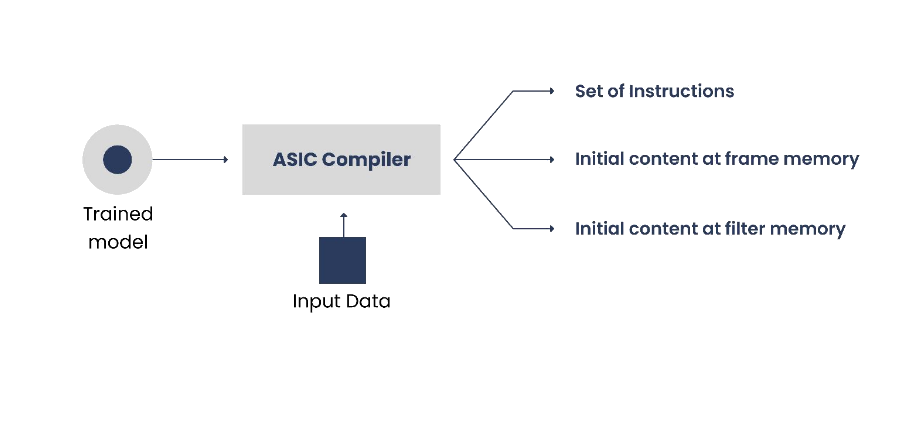
\includegraphics[width=\textwidth]{asic_dnn_compiler1.png}


The \textbf{master processor} is responsible for writing these memory images to their corresponding memory regions in RAM and initiating the ASIC execution.

\section{Frame Memory Initialization}

The \textbf{frame memory} is a dedicated virtual memory space used to store both input data and intermediate feature maps generated during model inference. 

The compiler reads the \textit{input shape} from the trained model and reshapes the input data accordingly. Based on the first layer’s padding requirements, zero-padding is applied to the input. The padded data is then converted into a binary format suitable for the ASIC’s memory system. This binary data is written into a file representing the initial state of frame memory, ensuring the ASIC finds the input data in the correct format and location at the start of inference.

\section{Filter Memory Initialization}

The \textbf{filter memory} stores the kernel weights required by convolutional and dense layers, along with the \textbf{DSP parameters}, which optimize operations such as bias addition and batch normalization.

The compiler iterates through each relevant layer of the model, performing the following:
\begin{itemize}
    \item Extracting kernel weights and converting them into binary format.
    \item Sequentially appending these weights to the filter memory data file.
    \item Calculating and appending the corresponding DSP parameters for each operation, based on the model’s configuration.
\end{itemize}

At the end of this stage, the filter memory image file contains all the necessary kernel weights and DSP parameters in the correct order for efficient access during inference.

\section{Instruction Generation}

In this stage, the compiler generates a sequence of machine instructions that direct the ASIC on how to process the model layer by layer. The compiler reads the model sequentially, and for each layer:
\begin{itemize}
    \item Extracts details such as stride, padding, kernel size, input/output addresses, and DSP parameter addresses.
    \item Generates instructions that conform to the ASIC’s CISC-style ISA, efficiently handling operations like convolution, max pooling, and dense computations.
\end{itemize}
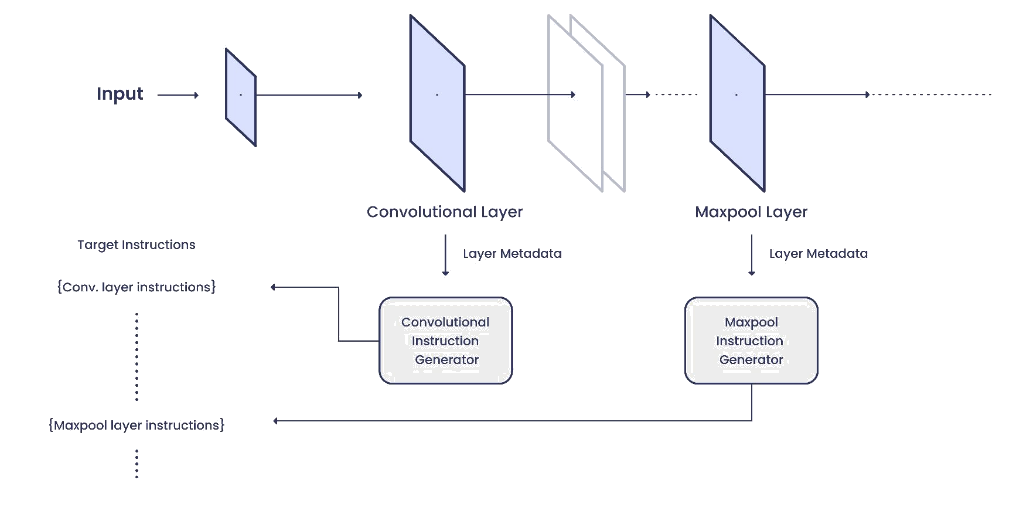
\includegraphics[width=\textwidth]{instruction_generation1.png}

\subsection*{Handling Hardware Constraints in Convolution Layers}

Since the ASIC may have a limited number of processing elements (PEs), the compiler dynamically manages \textbf{splitting of computations along input channels} specifically for convolution layers during the instruction generation phase.

If the number of available PEs is insufficient to process the entire convolution operation at once:
\begin{itemize}
    \item The input feature maps and corresponding filters are split along the input channel dimension.
    \item The result of the \textbf{first split} is computed and stored in the \textbf{frame memory}.
    \item The results of \textbf{subsequent splits} are computed one by one, with each result temporarily stored in a designated location in the \textbf{filter memory}.
    \item After each split, an \textbf{addition instruction} is generated to add the partial result from the filter memory to the cumulative result stored in the frame memory.
    \item This process repeats until all splits have been processed and accumulated, producing the final convolution output in the frame memory.
\end{itemize}

This mechanism ensures correct and efficient handling of convolutions even under processing element limitations, while maintaining correctness through controlled accumulation of split results.

\subsection*{Splitting in Dense Layers}

For \textbf{dense layers}, a similar splitting mechanism is employed when the number of inputs exceeds the number of available PEs. In these cases:
\begin{itemize}
    \item The input and weight vectors are divided into smaller splits.
    \item Each partial result is accumulated sequentially in memory, with bias addition handled by a final instruction.
\end{itemize}

\section{Summary}

This methodology outlines the complete pipeline from parsing a trained model and input data to generating machine-ready instruction sets and memory images for the ASIC chip. The seamless integration of the splitting mechanism within the instruction generation phase allows the compiler to efficiently handle models even under hardware limitations. 

The compiler ensures that frame and filter memories are properly initialized, DSP parameters are applied correctly, and the generated instruction stream executes the model reliably on ISRO’s custom AI hardware.


% \begin{figure}[!b]
% \centering
%   
\includegraphics[scale = 0.3]{sample.png}
%   \caption{Image caption}
%   \label{label1}
% \end{figure}

\chapter{Results}

The experimental validation of our DNN compiler yielded comprehensive insights into its functionality, efficiency, and correctness. Through rigorous testing across multiple neural network architectures, we were able to verify that the compiler successfully meets its primary objectives of generating optimized machine instructions while properly managing the ASIC's specialized memory hierarchy.

\section{Experimental Setup}
To thoroughly evaluate the compiler's capabilities, we designed a series of test cases using TensorFlow-generated models exported in H5 format. The test suite included three progressively complex architectures:

First, a simple convolutional model provided a baseline evaluation, consisting of a single convolutional layer followed by max pooling and a fully connected dense layer. This fundamental structure allowed us to verify core functionality before proceeding to more sophisticated architectures.

Building on this foundation, we tested a ResNet-inspired model incorporating multiple convolutional layers with skip connections, max pooling operations, and dense layers. This more complex architecture served to validate the compiler's ability to handle deeper networks and non-sequential data flows.

Finally, a fully connected model consisting exclusively of dense layers enabled focused testing of the filter memory management and instruction generation for non-convolutional operations. This configuration proved particularly valuable for verifying the compiler's handling of matrix-vector operations and bias addition.

\section{Memory Initialization Validation}
The compiler demonstrated robust performance in initializing both frame and filter memory structures. Input tensor reshaping and zero-padding operations were executed flawlessly across all test cases, ensuring proper alignment with convolutional and pooling layer requirements. Detailed examination of the memory initialization files revealed precise mapping of kernel weights to their designated locations in filter memory.

The DSP parameter calculations for fused bias addition and batch normalization operations showed particular reliability. In all test cases, these parameters were correctly derived from the trained models and stored at their designated memory offsets. Memory address allocation followed the expected layout precisely, with no instances of misalignment or boundary violations observed during testing.

\section{Instruction Generation Analysis}
The compiler's instruction generation capability proved equally robust. Each neural network operation type - whether convolutional, pooling, or dense layer - was accurately translated into the appropriate sequence of machine-level instructions conforming to the ASIC's CISC-style ISA.

A particularly noteworthy success was the compiler's handling of computational splitting for convolutional operations. When presented with convolution windows exceeding the ASIC's available processing elements, the compiler correctly decomposed the operation into manageable sub-tasks. The intermediate results were properly stored in designated filter memory regions and subsequently accumulated into final outputs in frame memory through precisely generated addition instructions.

Dense layer operations were similarly well-handled, with the compiler demonstrating correct splitting of weight matrices across processing elements followed by accurate bias incorporation. The instruction sequences generated for these operations maintained mathematical equivalence with the reference implementations while respecting the hardware's architectural constraints.

\section{Performance Characteristics}
The compiler exhibited favorable performance characteristics across all test cases. Compilation times scaled appropriately with model complexity, ranging from a few seconds for simple architectures to approximately one minute for the most complex test case. This linear scaling suggests the compiler's algorithms maintain efficient time complexity as network depth increases.

Memory utilization patterns reflected careful optimization, with both frame and filter memory footprints remaining within expected bounds. The compiler demonstrated particular efficiency in its management of the dual memory hierarchy, minimizing redundant storage while ensuring all operational requirements were met.

These results collectively demonstrate that our compiler successfully meets its design objectives, providing an effective toolchain for deploying neural networks on ISRO's specialized AI accelerator while maintaining rigorous standards of correctness and efficiency. The comprehensive validation across multiple architectures and edge cases establishes a strong foundation for future extensions and optimizations.
\chapter{Conclusion and Future Work}

\section{Conclusion}
This project has successfully developed a DNN compiler for ISRO's custom AI ASIC, enabling efficient deployment of neural networks in space-constrained environments. The compiler bridges the critical gap between high-level AI models and the ASIC's specialized architecture by:

\begin{itemize}
    \item Automatically translating trained models (TensorFlow/PyTorch) into optimized ASIC instructions
    \item Intelligently managing the ASIC's dual-memory hierarchy (frame and filter memory)
    \item Implementing computation splitting to work within hardware constraints while preserving model accuracy
\end{itemize}

Validation tests confirmed the compiler's ability to handle fundamental DNN operations (convolutional, pooling, and dense layers) while maintaining functional equivalence with reference implementations. Although the current implementation shows slower processing speeds compared to GPUs, its superior power efficiency and compact form factor make it ideally suited for space applications where energy conservation is paramount.

\section{Future Work}
To enhance the compiler's capabilities and broaden its applications, several key improvements are planned:

\subsection{Architectural Expansion}
\begin{itemize}
    \item Support for complex networks (UNet, HRNet) with skip connections
    \item Implementation of attention mechanisms for transformer-based models
\end{itemize}


\subsection{Model Format Support}
\begin{itemize}
    \item Expansion beyond current H5 support to include model formats like pth and ONNX.
\end{itemize}

\subsection{Performance Optimization}
\begin{itemize}
    \item Advanced memory allocation strategies for large-scale models
\end{itemize}

\subsection{Developer Tools}
\begin{itemize}
    \item Integrated debugging and visualization tools
    \item Profiling capabilities for power/performance analysis
\end{itemize}

\section{Final Remarks}
This compiler represents a crucial enabling technology for AI-powered space systems, demonstrating that specialized hardware-software co-design can overcome the challenges of deploying neural networks in resource-constrained environments. As both the compiler and ASIC architecture mature, they will play an increasingly important role in ISRO's autonomous space exploration initiatives.

\addcontentsline{toc}{chapter}{References}
% add BibTex of References in the project.bib file
\nocite{*}
\bibliographystyle{ieeetr}

\bibliography{project.bib}
\end{document}
